\documentclass[nojss]{jss}

%%%%%%%%%%%%%%%%%%%%%%%%%%%%%%
%% declarations for jss.cls %%%%%%%%%%%%%%%%%%%%%%%%%%%%%%%%%%%%%%%%%%
%%%%%%%%%%%%%%%%%%%%%%%%%%%%%%
% library(cacheSweave)
% Sweave("c060_vignette.Rnw", driver = cacheSweaveDriver)
% tools::texi2dvi("c060_vignette.tex", pdf=TRUE)
%%%%%%our stuff
\usepackage{graphicx}
\usepackage{mathptmx}      % use Times fonts if available on your TeX system
\usepackage[authoryear]{natbib}
\usepackage{amsmath}
\usepackage{amssymb}
\usepackage{amsfonts}
\usepackage{hyperref}
\usepackage{longtable}
\usepackage{color}
\usepackage{float}
%usepackage{pst-all}

% please place your own definitions here and don't use \def but
% \newcommand{}{}
%\newcommand{\Scmd}[1]{\texttt{#1}} % For R/ S commands
\definecolor{red}{rgb}{1,0.4,0.4}
\definecolor{blue}{rgb}{0.4,0.4,1}
\definecolor{green}{rgb}{0,0.5,0}
\definecolor{gradbegin}{rgb}{0.6,0.1,0.6} % purple

\author{Martin Sill\\
\And Thomas Hielscher\\ \hspace{3.95 cm} Division of Biostatistics (C060) \\  \hspace{4.3 cm} German Cancer Research Center, Heidelberg
\And Natalia Becker\\
\And Manuela Zucknick\\}
\title{\pkg{c060}: Extended Inference with Lasso and Elastic-Net Regularized Cox and Generalized Linear Models}

%% for pretty printing and a nice hypersummary also set:
\Plainauthor{Martin Sill, Thomas Hielscher, Natalia Becker, Manuela Zucknick} %% comma-separated
\Plaintitle{\pkg{c060}: Extended Inference with Lasso and Elastic-Net Regularized Cox and Generalized Linear Models} %% without formatting
\Shorttitle{\pkg{c060}: Extended Inference with Regularized Cox and Generalized Linear Models} %% a short title (if necessary)

%% an abstract and keywords
\Abstract{
We have developed the \proglang{R} package \pkg{c060} \citep{c060} with the aim of improving \proglang{R} software functionality for high-dimensional risk prediction modelling,
e.g., for prognostic modelling of survival data using high-throughput genomic data. 
Penalized regression models provide a statistically appealing way of building risk prediction models from high-dimensional data.
The popular CRAN package \pkg{glmnet} package \citep{glmnet} implements an efficient algorithm for fitting penalized Cox and generalized linear models.
However, in practical applications the data analysis will typically not stop at the point where the model has been fitted. One is for example often interested in the stability
of selected features and in assessing the prediction performance of a model and we provide functions to deal with both of these tasks. Our \proglang{R} functions are computationally
efficient and offer the possibility of speeding up computing time through parallel computing. Another feature which can drastically reduce computing time is an efficient interval-search algorithm,
which we have implemented for selecting the optimal parameter combination for elastic net penalties. These functions have been useful in our daily work at the
Biostatistics department (C060) of the German Cancer Research Center where prognostic modelling of patient survival data is of particular interest.
Although we focus on a survival data application of penalized Cox models in this article, the functions in our \proglang{R} package are in general applicable to all types of regression models implemented in the \pkg{glmnet} package, with the exception of prediction error curves, which are specific to time-to-event data.

}
\Keywords{\pkg{glmnet}, penalized log-likelihood method, stability selection, interval search, prediction error}
\Plainkeywords{glmnet, penalized log-likelihood method, stability selection, interval search, prediction error} %% without formatting
%% at least one keyword must be supplied

%% publication information
%% NOTE: Typically, this can be left commented and will be filled out by the technical editor
%% \Volume{50}
%% \Issue{9}
%% \Month{June}
%% \Year{2012}
%% \Submitdate{2012-06-04}
%% \Acceptdate{2012-06-04}

%% The address of (at least) one author should be given
%% in the following format:
\Address{
  Martin Sill\\
  Division of Biostatistics\\
  DKFZ\\
  German Cancer Research Center\\
  69120 Heidelberg, Germany\\
  E-mail: \email{m.sill@dkfz.de}\\
  URL: \url{http://www.dkfz.de/en/biostatistics}
}
%% It is also possible to add a telephone and fax number
%% before the e-mail in the following format:
%% Telephone: +43/512/507-7103
%% Fax: +43/512/507-2851

%% for those who use Sweave please include the following line (with % symbols):
%% need no 
\usepackage{Sweave}

%% end of declarations %%%%%%%%%%%%%%%%%%%%%%%%%%%%%%%%%%%%%%%%%%%%%%%


\begin{document}
\Sconcordance{concordance:c060_vignette.tex:c060_vignette.Rnw:%
1 213 1 1 31 1 28 1 8 12 1 1 3 5 0 1 2 4 1 1 2 1 0 1 2 1 0 2 1 %
4 0 1 2 4 1 1 7 1 2 4 0 1 1 1 3 2 1 1 2 1 0 1 1 3 0 1 2 1 1 2 %
2 21 1 1 12 14 0 1 2 3 1 1 3 5 0 1 2 1 1 1 3 1 2 17 1 1 2 1 0 %
1 1 1 2 4 0 1 2 3 1 1 2 8 0 1 2 4 1 2 2 14 1 1 2 1 0 1 1 1 2 1 %
1 1 2 2 1 3 0 1 2 4 1 1 10 12 0 1 2 1 1 1 23 1 1 1 2 21 0 1 2 %
3 1 1 6 2 1 1 5 2 1 1 2 5 0 1 2 12 1 1 2 5 0 1 2 58 1}

%\SweaveOpts{concordance=TRUE}
%\SweaveOpts{concordance=TRUE}

\section{Introduction}
\label{intro}

Penalized regression models provide a statistically appealing method to build prediction models from high-dimensional data sources, where it is the aim to simultaneously select features and to fit the model \citep{fan2010,benner2010}. Since the introduction of the lasso for linear regression models \citep{tibshirani96}, the methodology has been extended to generalized linear regression models and time-to-event endpoints \citep{tibshirani97} among others. In addition to the well-known $L_1$-norm (lasso) and $L_2$-norm (ridge) penalty functions, various other penalties have been proposed in recent years to select features and/or estimate their effects. In particular, we will use the elastic net penalty function \citep{zou05}, which is a linear combination of the $L_1$- and $L_2$-norms.

With ever increasing data, the properties of the algorithm used for fitting the model have become almost as important as the statistical model itself. 
\citet{FHT2010} proposed a coordinate descent algorithm for generalized linear regression models, which has since then been extended to penalized Cox proportional hazards (PH) regression models \citep{simon2011}. Due to its efficiency this algorithm is considered one of the state-of-the-art
approaches to estimate penalized regression models with lasso, ridge or elastic net penalty terms, especially in high-dimensional data scenarios. 
First references about coordinate descent algorithms date back to \citet{Fu98}. %and \citet{friedman07}.

This algorithm has been implemented in \proglang{R} \citep{R11} in the \pkg{glmnet} package \citep{glmnet}. The package provides functions to tune and fit regression models, plot the results, and make predictions. However, in practical applications, where often an independent validation data set is lacking, some additional features and routines are desirable as part of a complete data analysis. We have assembled some functions that enhance the existing functionality of the \pkg{glmnet} package or
allow to use it within the framework of other existing \proglang{R} packages. These functions have been useful in our daily work at the
Biostatistics department (C060) of the German Cancer Research Center where prognostic modelling of patient survival data is of particular interest. Therefore, for illustration purposes we focus on penalized Cox PH regression models in this article. But the \proglang{R} functions are generally applicable to all types of regression models implemented in the \pkg{glmnet} package.

Computational efficiency is an important requirement of the software to make applications feasible for real-life data analysis tasks in fields such as molecular oncology, where one aims to develop sparse risk prediction models based on very large numbers of molecular features measured with high-throughput technologies such as microarrays or next-generation sequencing. Therefore, we provide functionality to speed up computations, in particular through parallel computing.

We provide \proglang{R} functions to perform stability selection \citep{MeinshausenBuehlmann2010} in a computationally efficient way which allows to select the most stable features at a given Type I error level. We have also implemented an approach to select the optimal parameter combination ($\alpha$, $\lambda$) for elastic net penalties using an interval-search algorithm \citep{froehlich2005} which is often faster and more accurate than a standard grid search \citep{Jones1998}. Another very useful addition for real-life applications of \pkg{glmnet} for building risk-prediction models is the provision of wrapper functions to allow the computation of resampling-based prediction errors within the framework of the \proglang{R} package \pkg{peperr} \citep{Porz2009}. The \pkg{peperr} package makes it computationally feasible to assess the
predictive accuracy of a penalized regression model via resampling methods even for very large-scale applications by employing parallel computing. We also provide the possibility to speed up stability selection by parallel computing using the functionalities of the \proglang{R} base package \pkg{parallel} \citep{R11}.

Stability selection and interval search are currently defined for Gaussian, binomial, Poisson, multinomial and Cox models,  prediction error curves for Cox models and classification errors for
binomial models. Since all functions are basically wrapped around the \pkg{glmnet} fitting or cross-validation function calls, the type of response is always specified by the \code{family} argument. 

The software is available as \proglang{R} package \pkg{c060} on CRAN (URL \url{http://cran.r-project.org/web/packages/c060/}, version 0.2-3 at time of manuscript publication) and on R-forge (URL \url{https://r-forge.r-project.org/projects/c060/}, version 0.2-3 at the time of publication).

\section{Methods and algorithms}

\subsection{Penalized generalized linear models and Cox models}\label{methods:penalized}
An efficient implementation for fitting generalized linear models and Cox proportional hazards models with regularization by the lasso or elastic net penalty terms is provided by the \proglang{R} package \pkg{glmnet}. This implementation uses a coordinate descent algorithm for fitting the models for specified values of penalty parameters $\lambda > 0$ and $\alpha \in (0,1]$. The computation of an entire regularization path across a range of values $\Lambda = \{\lambda_1,\lambda_2...,\lambda_K\}$ at fixed $\alpha$ with \pkg{glmnet} is generally very fast, because previously computed solutions for $\{\lambda_1,...,\lambda_{k-1}\}$ are used as 'hot' starting values for the computation of $\lambda_k$. This implies that it is often more efficient to compute the models for the entire regularization path of $\Lambda$ rather than just individual models. We use this feature in all of our implemented algorithms to make most use of the computational speed of \pkg{glmnet}.

Models are fitted by maximizing the penalized log-likelihood function for generalized linear models and the penalized partial log-likelihood for Cox models. The penalized (partial) log-likelihood function is given by
\begin{equation}\label{pen.part.likelihood}
l_n(\boldsymbol\beta)- \sum_{j=1}^p  p_{\alpha,\lambda}(|\beta_j|)
\end{equation}
where $l_n(\boldsymbol\beta)$ denotes the (partial) log-likelihood given $n$ observations.
The dimension of the parameter vector $\boldsymbol\beta$ is $p$ and $p_{\alpha,\lambda}(|\cdot|)$ is the penalty function with tuning parameters $\lambda$ and $\alpha$.

Cross-validation can be performed to decide which model, i.e., which penalty parameter values, to choose by using the negative cross-validated penalized (partial) log-likelihood as the loss function. Actually, within the \pkg{glmnet} package, the penalized (partial) log-likelihood deviance is used as the loss function rather than the log-likelihood function itself. The deviance is equal to -2 times the log-likelihood ratio of the model of interest compared to the saturated model, which has one free parameter per observation. Obviously, both versions will result in the same optimization result.

\subsection{$L_2$-penalized Cox regression}
Penalized maximum likelihood estimation in Cox regression with the ridge penalty
\begin{equation}\label{ridge}
p_{\lambda}(|\beta_j|)=\lambda\beta_j^2
\end{equation}
was introduced by \citet{verweij94}.
The ridge penalty results in parameter estimates that are biased towards zero, but does not set values exactly to zero, and hence does not perform feature selection.
On the other hand, it has been found to produce models with good prediction performance in high-dimensional genomic applications \citep[e.g.,][]{bovelstad07}, in particular if predictors are highly correlated.

\subsection{$L_1$-penalized Cox regression}
\Citet{tibshirani97} proposed to use an $L_1$-penalized Cox model with
\begin{equation}
p_{\lambda}(|\beta_j|)=\lambda | \beta_j |
\end{equation}
and described a technique, called the lasso for ``least absolute shrinkage and selection operator'', for parameter estimation.
The $L_1$-penalty has the advantage over the $L_2$-penalty of shrinking some of the coefficients to zero, i.e., it performs automatic feature selection.

\subsection{The elastic net}
\Citet{zou05} introduced the elastic net, which employs a combination of the $L_1$- and $L_2$-penalty. Like lasso the elastic net performs automatic feature selection by setting some coefficient estimates to zero.
But the additional $L_2$-penalty term distributes the weight to more features, so that the elastic net tends to select more features than the lasso. 
This is especially the case in situations with high correlation, since the lasso would select only one feature of a set of perfectly correlated features, while the ridge penalty would give them equal weight.

Throughout this manuscript we use the same parametrization of the elastic net penalty function as the formulation used in the \pkg{glmnet} package:
  \begin{equation}\label{enet2}
p_{\alpha,\lambda}(|\beta_j|)= \lambda\times (\alpha |\beta_j| + (1-\alpha)\frac{1}{2} \beta_j^2).
\end{equation}
Here, $\alpha \in (0,1]$ determines the influence of the $L_1$ penalty relative to the $L_2$ penalty. Small $\alpha$ values will result in models with many features, getting closer to the non-sparse ridge solution as $\alpha$ tends to zero.

\subsubsection{The interval-search algorithm to select the optimal elastic net parameter combination}
The elastic net penalty function contains two tuning parameters which are data-dependent and hence cannot be set to some \emph{a priori} values. The challenge is to find a set of tuning parameters $\left(\alpha,\lambda\right)$, for which the k-fold cross-validated loss function of the model is minimal.

The commonly used fixed grid search has its major disadvantage in the need to systematically compute the penalized log likelihood deviance at each point of the grid, which implies that the grid density affects the accuracy and the time complexity of the algorithm. Furthermore, the choice of the grid is highly arbitrary and the solution depends on the choice of grid as well as on grid density. 

\Citet{froehlich2005} proposed an efficient algorithm for finding a global optimum on the tuning parameter space 
called Efficient Parameter Selection via Global Optimization (EPSGO). The main idea of the algorithm is to treat the task of finding the optimal tuning parameter values as a global optimization problem. For that purpose one learns a Gaussian process model of the loss function surface in parameter space and samples systematically at points where the so-called expected improvement criterion reaches the maximum. 

The interval search can be divided into two phases. In the initial phase, a set of uniformly distributed points is randomly selected throughout the parameter space. Then, in the iteration phase, the algorithm learns the Gaussian process model from the points which have already been visited. By adding new points one updates the Gaussian process model.
New points in the parameter space are sampled by using the expected improvement criterion as described by \citet{Jones1998}. The EPSGO algorithm stops when one of the stopping criteria is met, i.e., if either convergence of the algorithm has been reached or if there was no change in the solution during the last ten iterations.

\Citet{froehlich2005} showed that the algorithm is robust against local minima. 
One can observe an immense improvement in the training time for the Gaussian process model compared to more commonly used fixed grid search methods \citep{froehlich2005}. This is because the number of training points for the Gaussian process (and hence the number of evaluations of the loss function surface of the regression model) mainly depends on the dimensionality of the tuning parameter space, which is very small compared to the number of training points on the grid.

Summing up, the EPSGO algorithm provides two main advantages when compared to grid search methods: 
\begin{itemize}
\item Robustness against starting values: EPSGO solutions are not dependent on an arbitrary choice of a grid.
\item Scalability of accuracy improvements: The accuracy of EPSGO solutions can be easily improved without the need for a massive increase in computing time implied by an increase in the grid density.
\end{itemize}

\subsection{Stability selection}
The penalized regression models that we have described above are typically used to find sparse models with good predictive performance. In contrast, the stability selection proposed by \citet{MeinshausenBuehlmann2010} aims to find stable features which show strong association with the outcome. 
The stability selection is a general approach that combines feature selection methods such as $L_1$ penalized models with resampling. By applying the corresponding feature selection method to subsamples that were drawn without replacement, selection probabilities for each feature can be estimated as the proportion of subsamples where the feature is included in the fitted model. These selection probabilities are used to define a set of stable features. \citet{MeinshausenBuehlmann2010} provide a theoretical framework for controlling Type I error rates of falsely assigning features to the estimated set of stable features. The selection probability of each feature along the regularization path, e.g., along the range of possible penalization parameters $\Lambda=\{\lambda_1,\lambda_2...,\lambda_K\}$, is called stability path.
Given an arbitrary threshold $\pi_{thr} \in (0.5,1)$ and the set of penalization parameters $\Lambda$, the set of stable features estimated with stability selection is:
\begin{equation} 
 \hat{S}_{\beta}^{stable}=\left\{j: \max_{\lambda_{k} \in \Lambda} \hat{\Pi}_{j}^{\lambda_{k}} \geq \pi_{thr} \right\},
\end{equation}
where $\hat{\Pi}_{j}^{\lambda_{k}}$ denotes the estimated selection probability of the $j$th feature at $\lambda_k$. 
Then according to Theorem 1 in \citet{MeinshausenBuehlmann2010}, the expected number of falsely selected features $E(V)$ will be bounded by:
\begin{equation}\label{stab}
E(V) \leq \frac{1}{(2\pi_{thr}-1)} \frac{q^{2}_{\Lambda}}{p},
\end{equation}
where $q_{\Lambda}$ is the average of the number of non-zero coefficients with respect to the drawn subsamples.  
Equation~\ref{stab} shows that the bound on expected number of falsely selected features can be decreased by either reducing the average number of selected features $q_{\Lambda}$ or by increasing the threshold $\pi_{thr}$. Suppose that $\pi_{thr}$ is fixed, then $E(V)$ can be controlled by limiting $q_{\Lambda}$ by the length of the regularization path $\Lambda$. In multiple testing the expected number of falsely selected features is also known as the per-family error rate (PFER) and if divided by the total number of features $p$ will become the per-comparison error rate (PCER) \citep{Dudoit2003}. The stability selection allows to control these Type I error rates. For instance, suppose the threshold $\pi_{thr} = 0.8$ is fixed, then choosing $\Lambda$ such that $q_{\Lambda} \leq \sqrt{0.6p}$ will control $E(V)\leq 1$. Moreover, choosing $\Lambda$ so that $q_{\Lambda} \leq \sqrt{0.6p\alpha}$ will control the family-wise error rate (FWER) at level $\alpha$, $P(V>0) \leq \alpha$.
As mentioned before, according to \citet{FHT2010} the coordinate descent algorithm implemented in the \pkg{glmnet} package is most efficient regarding the computational time, when used to calculate the full regularization path. To utilize this property our algorithm calculates the stability path by first generating subsets by subsampling and then calculating for each subsample the regularization path using the coordinate descent algorithm. The resulting regularization paths are then averaged to form the stability path. Furthermore, since the calculations of the regularization paths for each subset are independent of each other, the algorithm can easily be parallelized using the package \pkg{parallel}. %In parallel computing such easily to parallelize  embarrassingly parallel computations.    

\subsection{Prediction error curves for survival models}

The time-dependent Brier score \citep{graf99} can be used to assess and compare the prediction accuracy of prognostic models for time-to-event endpoints.
The Brier score at time point $t$ is a weighted mean squared error between predicted survival probability and observed survival status.
Weighting depends on the estimated censoring distribution to account for the observations under risk \citep{gerds2006}. Computing the error for each time point over the entire follow-up horizon yields a prediction error curve. As a reference we use prediction errors based on the Kaplan-Meier curves estimated without any covariate information. 

The empirical time-dependent Brier score $BS(t)$ is defined as a function of time $t > 0$ by
\[
BS(t) = \frac{1}{n}\sum_{i=1}^{n}{\left[\frac{\hat{S}(t|x_i)^2I(t_i\leq t \wedge \delta_i=1)}{\hat{G}(t_i)} + \frac{(1-\hat{S}(t|x_i))^2I(t_i>t)}{\hat{G}(t)}\right]},
\]
with individual survival time $t_i$, censoring indicator $\delta_i$ and estimated survival probability $\hat{S}(t|x_i)$ at time $t$ based on the prognostic model given covariate values $x_i$ for subject $i$ out of $n$ patients \citep{graf99}.
$\hat G(t)$ denotes the Kaplan-Meier estimate of the censoring distribution at time $t$, which is based on the observations $(t_i; 1-\delta_i$), $i = 1,...,n$. $I$ signifies the indicator function. 

In case no independent validation data are available, resampling-based prediction error curves are used to adequately assess the model's prediction accuracy. The $.632+$ bootstrap estimator \citep{efron1997} is commonly used for these applications, which is a weighted mean of the apparent error and the average out-of-bag bootstrap error. For the apparent error  the same data is used to develop the prognostic model and assess its performance. Due to overfitting, this error is far too optimistic, particularly with high-dimensional data. The average out-of-bag bootstrap error is too conservative since only a proportion of the entire data is used to develop the prognostic model in each bootstrap run. 
The $.632+$ estimator balances both estimators, and additionally accounts for the relative overfitting based on the no-information error rate.
Further, in our application the $.632+$ bootstrap estimator is calculated based on subsampling (without replacement) rather than classical bootstrap sampling with replacement, as that has been demonstrated to lead to more accurate estimates in a high-dimensional context \citep{BS2008}.




\section{Application and demonstration of software}

\subsection{Data set}
\nocite{metzeler08}
In the following we will demonstrate the use of the functions provided in the \pkg{c060} package in an application to a gene expression data set and corresponding clinical data of cytogenetically normal acute myeloid leukemia (AML) patients \citep{metzeler08}. The data can be accessed from the Gene Expression Omnibus (GEO) data repository (\url{http://www.ncbi.nlm.nih.gov/geo}) by the National Center for Biotechnology Information (NCBI). We find the data set under GEO accession number GSE12417. To simulate the typical situation that only one data set is available for model training and evaluation, we only use the data set that was used as validation data in the original publication. This data set contains gene expression data for 79 patient samples measured with Affymetrix HG-U133 Plus 2.0 microarrays. The median survival time of these patients was 17.6 months with a censoring rate of 40\%.

For the sake of convenience we reduce the total number of 54675 gene expression features that have been measured with the Affymetrix HG-U133 Plus 2.0 microarray technology to the top 10000 features with largest variance across all 79 samples. For all computations the data set is stored as an \code{ExpressionSet} (from Bioconductor package \pkg{Biobase} \citep{Bioconductor}) called \code{eset}. The gene expression data matrix can be accessed through the call \code{exprs(eset)} and overall survival data and other patient-specific data (e.g., patient age) are stored within the \code{phenoData} object \code{pData(eset)}. Overall survival times are stored in the variable \code{os}, the corresponding survival status variable is called \code{os_status} and the patient age variable is \code{age}.

\subsection{Starting off: Fitting the lasso-penalized Cox model} 
Our goal is to develop a prognostic model for patient overall survival based on the gene expression data. The purpose of this modelling exercise is not just to fit a prognostic model that is capable of predicting overall survival rates, but we also want to find out which gene expression features are most relevant for this task. Traditionally, this problem is solved by feature selection methods and we start our data analysis exercise by fitting the lasso-penalized Cox model, which provides automatic feature selection.

We can apply the \code{glmnet} function to fit a lasso-penalized Cox model to the AML data set. The function call with default penalty parameter settings will fit the lasso model for 100 $\lambda$ values within a data-derived range of values:
\begin{Schunk}
\begin{Sinput}
R> fit <- glmnet(y=Surv(pData(eset)$os, pData(eset)$os_status), 
+                x=t(exprs(eset)), family="cox")
\end{Sinput}
\end{Schunk}
 
In order to determine the optimal lasso penalty parameter value, we perform 10-fold cross-validation using the \code{cv.glmnet} function.

\begin{figure}[H]
\begin{center}
\begin{Schunk}
\begin{Sinput}
R> set.seed(1234)
R> cvres <- cv.glmnet(y=Surv(pData(eset)$os, pData(eset)$os_status), 
+                     x=t(exprs(eset)), family="cox", nfolds=10)
R> res <- cvres$glmnet.fit
R> plot(cvres)
\end{Sinput}
\end{Schunk}
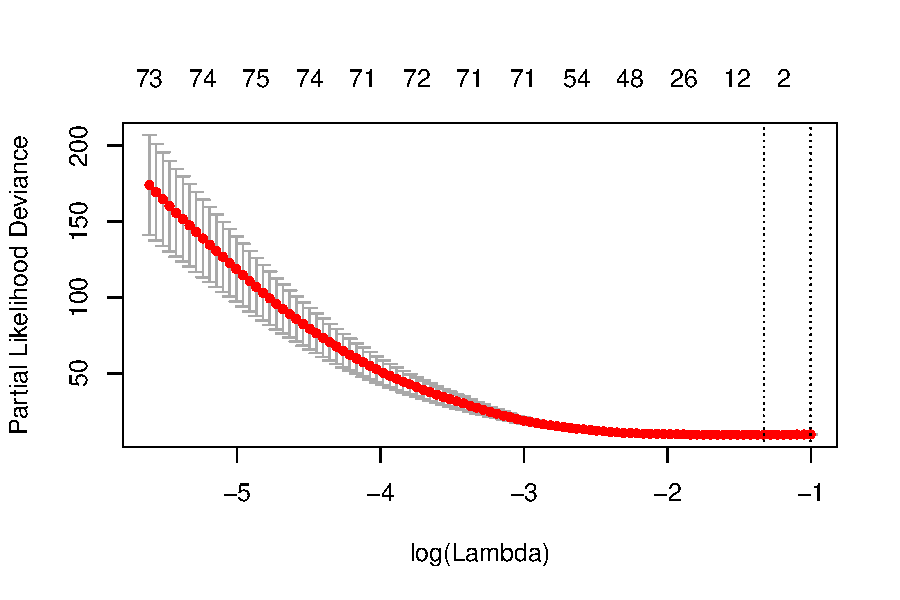
\includegraphics{c060_vignette-glmnet}
\end{center}
\caption{Cross-validated partial log-likelihood deviance, including upper and lower standard deviations, as a function of $\log{\lambda}$ for the AML data set. The dotted vertical lines indicate the $\lambda$ values with minimal deviance (left) and with the largest $\lambda$ value within one standard deviation of the minimal deviance (right).}
\label{fig:cvlasso}
\end{figure}

The loss function, i.e., the cross-validated partial log-likelihood deviance, is shown in Figure~\ref{fig:cvlasso} including upper and lower standard deviations as a function of $\log{\lambda}$ for the AML data set. The penalty parameter value minimizing the loss function is $\lambda =$0.265 ($\log\lambda =$-1.329) and corresponds to a final lasso model with the following 5 selected features and corresponding lasso regression coefficient estimates:
\begin{Schunk}
\begin{Soutput}
  203640_at 204419_x_at 222462_s_at   226169_at   233371_at 
    -0.1134     -0.0166      0.2742      0.0430     -0.0122 
\end{Soutput}
\end{Schunk}

The selected features are highlighted as red lines in the coefficient paths shown in Figure~\ref{fig:coefpath}, which illustrate the development of the regression coefficient estimates with increasing regularization. While the selected 5 features are the only features selected at the optimal $\lambda$ value, they do not remain among the features with largest effect sizes when the penalty is reduced and thus more and more coefficients start to enter the model. In fact, for 4 out of the 5 features the coefficient estimates go back down to zero for small values of $\log\lambda$, indicating that these features get replaced by other gene expression features in very large models.

\begin{Schunk}
\begin{Sinput}
R> cof <- coef(res, s=cvres$lambda.min)
R> Plot.coef.glmnet(cvfit=cvres, betas=rownames(cof)[which(cof!=0)])
\end{Sinput}
\end{Schunk}
\begin{figure}[H]
\begin{center}
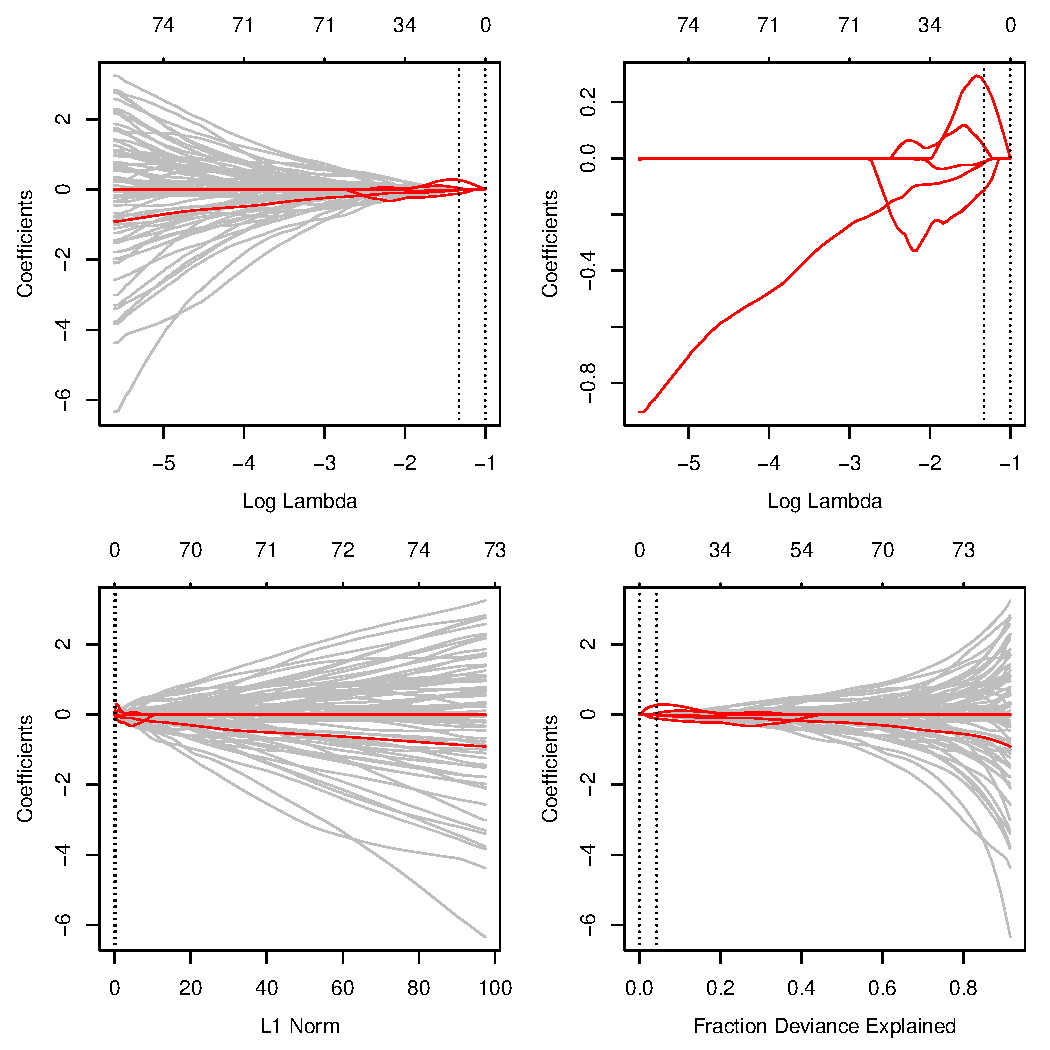
\includegraphics{c060_vignette-glmnet4}
\end{center}
\caption{\label{fig:coefpath}Coefficient paths for lasso-penalized Cox PH regression models applied to the AML data set. The features with highlighted paths have non-zero coefficients in the model with the optimal $\lambda$ value as determined by ten-fold cross-validation. %The dotted vertical have the same meaning as in Figure~\ref{fig:cvlasso}. 
The top plots show the coefficient path scaled to reflect $\log(\lambda)$ on the x-axis (top left: full path, top right: zoomed in to only show the selected features). The bottom plots show the coefficient paths relative to the $L_1$-norms of the estimated coefficient vector (left) and to the fraction of the null partial log-likelihood deviance explained (right).
The dotted vertical lines indicate the $\lambda$ values with minimal deviance and with the largest $\lambda$ value within one standard deviation of the minimal deviance.}
\end{figure}

\subsection{Assessment of prediction performance with resampling-based prediction errors}
\label{pec}

Once the final prognostic model is selected, the next task is to assess its prediction accuracy for future patients, where one is often particularly interested in a comparison with established clinico-pathological prognostic markers. In many applications no independent validation data set is available, and thus the same data set needs to be used to both develop and assess the prognostic model. This is especially problematic for high-dimensional data,
where the risk of overfitting is very high. Resampling-based methods can be used to unbiasedly estimate the predictive accuracy 
of the prognostic model in this situation. This is also called internal validation.

For this purpose the \proglang{R} package \pkg{peperr} \citep{Porz2009,peperr} provides a modular framework for survival and binary endpoints. %, i.e., prognostic and classification models. 
Wrapper functions for new or customized prediction model algorithms can be defined and passed to the generic call function \code{peperr}.  
In case of prognostic models for survival endpoints, algorithm-specific wrapper functions are required for model fitting, tuning and prediction. Wrapper functions for selected machine learning approaches are already implemented, but not yet for the \pkg{glmnet} package.

With the \pkg{peperr} package prediction accuracy of survival models is by default assessed with prediction error curves based on the time-dependent Brier score, but it is also possible to define and use customized accuracy measures. We have implemented additional wrapper functions for the \pkg{glmnet} algorithm for fitting (\code{fit.glmnet}) and tuning (\code{complexity.glmnet}) the model, and predicting survival probabilities (\code{predictProb.glmnet}) based on the fitted model and the estimated baseline hazard from the training data using the Breslow estimator. We here want to assess the prognostic value of the $L_1$-penalized Cox PH regression model fitted in the previous section. The $.632+$ subsampling-based bootstrap estimator is calculated using 1000 bootstrap samples. The \pkg{peperr} package is designed for high-dimensional covariates data and allows for various parallel computation setups.
Also, additional arguments can be passed directly to the \pkg{glmnet} call by specifying additional arguments for the corresponding fitting and/or tuning procedure.
Here, we include patient age as a mandatory feature, i.e., age is not subject to penalization, and 
run the calculation on 3 CPUs in parallel using a socket cluster setup. 

\begin{Schunk}
\begin{Sinput}
R> obj  <- peperr(response=Surv(pData(eset)$os, pData(eset)$os_status),
+                 x=data.frame(eset$age,t(exprs(eset))),
+                 fit.fun=fit.glmnet, args.fit=list(standardize=FALSE, family="cox",
+                 penalty.factor=rep(0:1, times=c(1,dim(eset)[1]))),
+                 complexity=complexity.glmnet, 
+                 args.complexity=list(standardize=FALSE, nfolds=10, family="cox", 
+                 penalty.factor=rep(0:1, times=c(1,dim(eset)[1]))),
+                 RNG="fixed", seed=0815, cpus=3, parallel=TRUE, clustertype="SOCK", 
+                 load.list=list(packages=c("c060")), 
+                 indices=resample.indices(n=dim(eset)[2],
+                 sample.n=1000, method="sub632"))
\end{Sinput}
\end{Schunk}

Bootstrap results can be visualized with the \code{plot.peperr} function from the \pkg{peperr} package showing the selected complexity parameters, 
out-of-bag prediction error curves as well as the prediction error integrated over time, and the predictive partial log-likelihood (PLL) values. In order to calculate the predictive PLL values again, an algorithm-specific wrapper (here \code{PLL.coxnet}) needs to be provided. In addition, we provide a slightly modified version of the prediction error curves plot function from the \pkg{peperr} package, which allows the display of the numbers of samples still at risk and pointwise bootstrap quantiles (\code{Plot.peperr.curves}) as shown in Figure~\ref{fig:pec}. By default, the $.632+$ bootstrap estimate is calculated and displayed. Optionally, one can additionally display the $.632$ estimator, the no-information error rate and the average out-of-bag bootstrap error in \code{Plot.peperr.curves} by setting the option \code{allErrors=TRUE}. \\

\begin{Schunk}
\begin{Sinput}
R> Plot.peperr.curves(obj, at.risk=TRUE, allErrors=FALSE, bootRuns=FALSE,
+                     bootQuants=TRUE, bootQuants.level=0.95, leg.cex=0.7)
\end{Sinput}
\end{Schunk}
\begin{figure}[t!]
\begin{center}
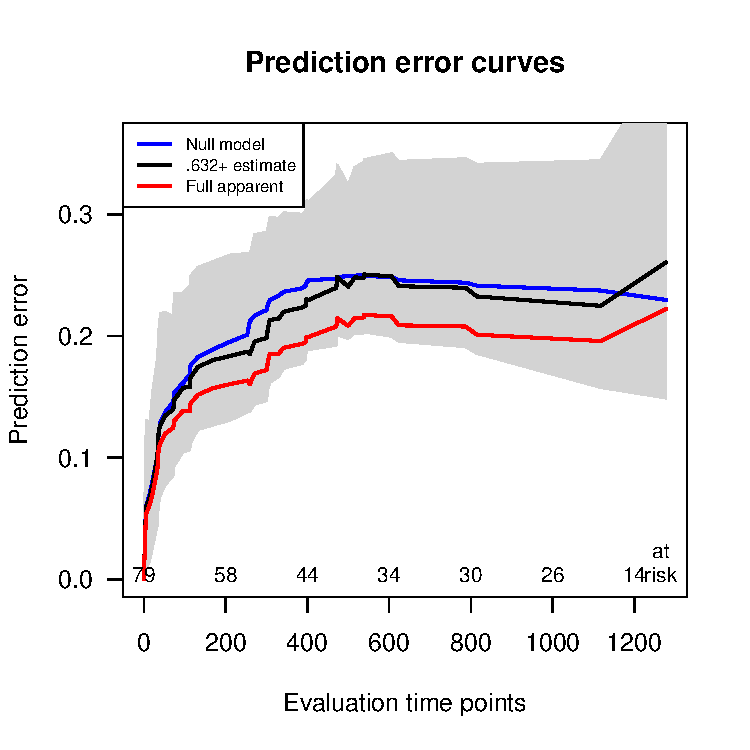
\includegraphics{c060_vignette-peperrPlot2}
\end{center}
\caption{Prediction error curves based on time-dependent Brier score for the lasso-penalized Cox PH regression model applied to the AML data set (evaluation time points reflect days). The gray area indicates the pointwise 2.5\% and 97.5\% quantiles of the 1000 out-of-bag bootstrap samples. The other lines show the prediction error curves of the null model (estimated by the Kaplan-Meier estimator without covariate information), the full apparent error estimates (i.e., the errors as estimated when applying the model to the entire training data set), and the .632+ bootstrap error estimates.}
\label{fig:pec}
\end{figure}

For classification models for binary endpoints, both tuning and fitting of the model are done with the same wrapper functions as used for the Cox regression. Model performance measures for classification tasks that are shipped with the \pkg{peperr} package are the misclassification rate and the Brier score. The predicted class probability is calculated within each generic performance function by calling the algorithm-specific predict function. Whenever a new algorithm/method is applied, the generic performance/aggregation function needs to be adapted accordingly. Therefore for binary responses, the \pkg{peperr} package does not provide quite the same modular flexibility as for time-to-event endpoints where prediction and performance assessment are done in separate functions.
We have extended the functionality of the \pkg{peperr} functions for calculating the Brier score (\code{aggregation.brier}) and the misclassification rate (\code{aggregation.misclass}) to allow their use with the \pkg{glmnet} algorithm. In addition, we have implemented the area under the receiver operating characteristic (ROC) curve (AUC) (\code{aggregation.auc}) as an alternative performance measure for binary response classifications. An example is included in the corresponding help file. For classification models, there are numerous alternative \proglang{R} and Bioconductor packages available to assess models fitted with \pkg{glmnet}. A good starting point is the package \pkg{caret} \citep{caret}.

An alternative implementation of the time-dependent Brier score for assessing the prognostic performance of prognostic models for time-to-event endpoints can be found in the package \pkg{pec} \citep{MIG2012}. The basic approach is similar to \pkg{peperr}, i.e. one has to define a wrapper for each fitting procedure in order to determine the estimated survival probabilities. Just as for \pkg{peperr}, no wrapper for \pkg{glmnet} is available yet with the \pkg{pec} package. The main difference of \pkg{peperr} compared to \pkg{pec} is that the tuning of the hyper-parameter and the fitting procedure are done in two separate steps, which reflects the usual workflow for high-dimensional data analysis better. While \pkg{pec} provides additional prediction accuracy measures for survival models, such as the time-dependent c-index, it cannot be used to assess classification models for binary endpoints. One strong point of the implementations of both \pkg{peperr} and \pkg{pec} is their easy-to-use setup for using resampling methods for internal validation. In addition to the use of prediction error curves and time-dependent Brier scores, another popular approach for assessing the prediction accuracy of survival models is the use of time-dependent ROC and AUC curves, for which many implementations exist, for example in \proglang{R} packages \pkg{timeROC} \citep{timeROC}, \pkg{survivalROC} \citep{survivalROC} and \pkg{risksetROC} \citep{risksetROC}. 

%\clearpage
\subsection{Stability selection}

So far implementations of stability selection can be found in the packages \pkg{s4vd}, \citep{s4vd,sill2011robust}, \pkg{mboost} \citep{mboost}, \pkg{lol} \citep{lol} and \pkg{BioMark} \citep{BioMark}. While in the package \pkg{s4vd} the stability selection is applied to sparse singular value decomposition in the context of biclustering, the \pkg{mboost} package offers stability selection for model based boosting. The implementation in the \pkg{lol} package is based on penalized generalized linear models and penalized Cox models available through the package \pkg{penalized} \citep{penalized}.  As both the \pkg{penalized} and the \pkg{glmnet} packages offer penalized models for survival, Poisson, binary and Gaussian response variables, the stability selection in \pkg{lol} is comparable to our implementation. Due to the computational efficiency of the coordinate descent algorithm in \pkg{glmnet} it is more appropriate for complex resampling methods like stability selection. Moreover, the code for the stability selection in the \pkg{lol} package is not yet parallelized and does not offer the possibility to compute the whole stability path. The \pkg{BioMark} package offers an implementation of stability selection for partial least squares (PLS), principal component regression (PCR), variable importance of projection (VIP) and logistic and Gaussian \pkg{glmnet} models. Until now the \pkg{BioMark} package allows only to calculate selection frequencies and does not provide type I error control nor the 'randomized lasso' as described in \citet{MeinshausenBuehlmann2010}. \\

Here we use stability selection to identify prognostic features, which have a relevant influence on the survival times of the patients in the AML data set, while controlling Type I errors to ensure that the features identified are truly associated with the survival times.
To calculate the stability path for the $L_1$-penalized Cox regression we use the function \code{stabpath} from our \proglang{R} package. Via the \code{weakness} argument of the function \code{stabpath} it is possible to induce additional randomization by reweighting the penalization of each feature. In brief, in each subsampling step the individual penalization of each feature is randomized such that it lies in the range of $[\lambda,\lambda/\kappa]$, where $\kappa$ is represented by the \code{weakness} parameter which indicates the amount of this additional randomization. The weights $w_{i},\cdots,w_{p}$ to replace each $\lambda_{i}$ by $\lambda_{i}/w_{i}$ are generated by sampling from a uniform distribution, i.e. $w_{i} \sim \mathcal{U}(\kappa,1)$. \citet{MeinshausenBuehlmann2010} call this additional randomization 'randomized lasso' and showed that it greatly improves the variable selection performance of the stability selection. The function \code{stabpath} draws subsets and calculates in parallel the stability path, e.g., the selection probabilities of each feature along the range of possible penalization parameter values. For parallelization we use the package \pkg{parallel}, which has been a base package since \proglang{R} version 2.14.0. On Unix-like systems the parallelization is done by forking via the function \code{mclapply} whereas under Windows systems socket clusters are used. 

\begin{Schunk}
\begin{Sinput}
R> y <- cbind(time=pData(eset)$os, status=pData(eset)$os_status)
R> set.seed(1234)
R> spath <- stabpath(y=y, x=t(exprs(eset)), mc.cores=2,
+                          family="cox", weakness=.8)
\end{Sinput}
\end{Schunk}


After calculating the stability path, the function \code{stabsel} can be called to estimate the stable set of features. Controlling a per-family error rate (PFER) of $1$, e.g., expecting one falsely selected feature, the estimated set of stable features comprises a single feature (with $\hat\Pi>0.6$).

\begin{Schunk}
\begin{Sinput}
R> stabsel(spath, error=1, type="pfer", pi_thr=0.6)$stable
\end{Sinput}
\begin{Soutput}
206932_at 
     2823 
\end{Soutput}
\end{Schunk}

Alternatively, the \code{stabsel} function allows to control the per-comparison wise error rate (PCER) and family-wise error rate (FWER). In addition, we provide a \code{plot} function to visualize the stability path. This function calls \code{stabsel} to estimate stable features and indicates them in the plot (Figure~\ref{stab:path}).

\begin{figure}[t!]
\begin{center}
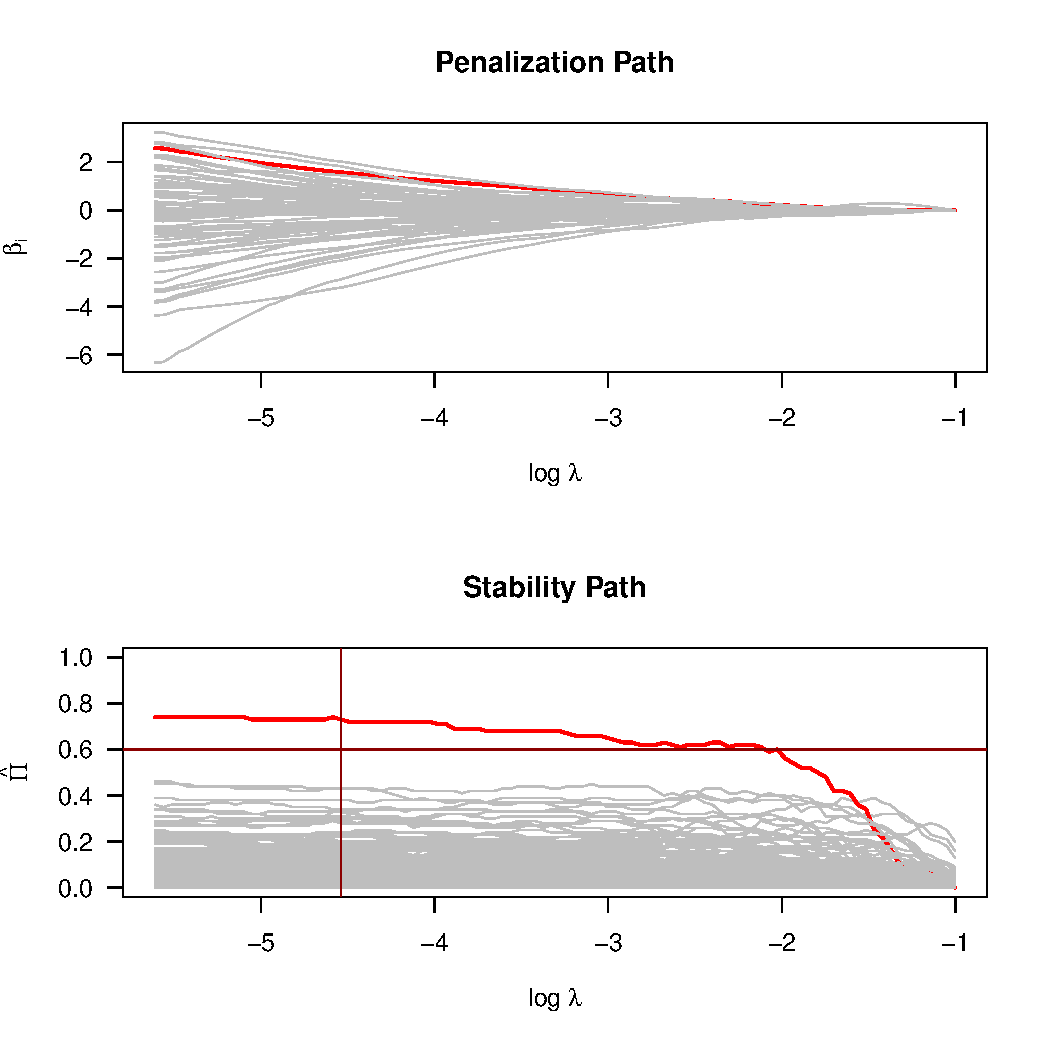
\includegraphics{c060_vignette-stabilitySelection3}
\end{center}
\caption{Coefficient and stability paths for lasso penalized Cox PH regression model applied to the AML data set. The feature with highlighted path is the only stable feature found by stability selection with PFER=1 and $\hat\Pi >0.6$.}
\label{stab:path}
\end{figure}

%\clearpage
\subsection{Parameter tuning for the elastic net Cox model}

In the previous sections we have seen that the lasso-penalized Cox model does not seem to perform very well in terms of predicting overall survival for the AML data set. 
The lasso model identified as the optimal model by 10-fold cross-validation is very sparse and contains only 5 features.
Furthermore, we have observed that these features are not very stable and 4 of them do not even remain in the set of selected features when the amount of regularization is decreased and more features start to enter the model.

In this section we fit an elastic net model instead of lasso to the same data set. As outlined above, fitting an elastic net model requires the simultaneous tuning of two parameters $\alpha$ and $\lambda$. For this computationally challenging task, we use the interval search algorithm in an efficient implementation in \proglang{R} function \code{EPSGO}. The EPSGO algorithm was originally implemented for support vector machines in the \proglang{R} package \pkg{penalizedSVM} \citep{becker2009,penSVM}. Here we provide a version for \code{glmnet} and in addition \code{summary} and \code{plot} functions to illustrate the interval search results.

The following code specifies the required objects and parameter values for optimizing the tuning parameters of the elastic net Cox model. The \code{balancedFolds} function splits the data into balanced folds for 10-fold cross-validation.
\begin{Schunk}
\begin{Sinput}
R>   x <- t(exprs(eset))
R>   y <- cbind(time=pData(eset)$os,status=pData(eset)$os_status)
R>   bounds <- t(data.frame(alpha=c(0, 1)))
R>   colnames(bounds)<-c("lower","upper")
R>   nfolds <- 10
R>   set.seed(1234)
R>   foldid <- balancedFolds(class.column.factor=y[,2], cross.outer=nfolds)
\end{Sinput}
\end{Schunk}

Usually, the task is to find a setting of tuning parameter values $\left(\alpha,\lambda\right)$, for which the 10-fold cross-validated penalized (partial) log likelihood deviance of the model is minimal. Here, however, the optimal $\lambda$ is chosen as the largest value of $\lambda$ such that the loss function is within one standard error of the minimum, which will result in a smaller model (a strategy suggested by the authors of the \pkg{glmnet} package). That is, for each given $\alpha$ an optimal $\lambda$ is found via the computation of the entire regularization path with the \code{glmnet} function with option \code{type.min ='lambda.1se'}.

The wrapper function \code{tune.glmnet.interval} calculates the (partial) log likelihood deviance of a model with given tuning parameter setting $\left(\alpha,\lambda\right)$.

\begin{Schunk}
\begin{Sinput}
R>   fit <- epsgo(Q.func="tune.glmnet.interval", 
+               bounds=bounds, 
+               parms.coding="none", 
+               seed = 1234, 
+               fminlower = -100,
+               x = x, y = y, family = "cox", 
+               foldid = foldid,
+               type.min = "lambda.1se",
+               type.measure = "deviance")
\end{Sinput}
\end{Schunk}



Summary information can be extracted from the \code{fit} object using the \code{summary} function.
\begin{Schunk}
\begin{Sinput}
R> sumint <- summary(fit, verbose=TRUE)
\end{Sinput}
\begin{Soutput}
Summary interval search 

show the first 5 out of 37 entries
    alpha    lambda deviance n.features
1 0.67605 0.4939544 9.711522          1
2 0.17194 1.5391420 9.662976         19
3 0.81895 0.4077635 9.708716          1
4 0.31188 0.9756053 9.699170          4
5 0.61671 0.5168716 9.700599          2

..............................

 Optimal parameters found are: 

alpha =  0.013 	 lambda =  14.722 deviance =  9.6329
\end{Soutput}
\end{Schunk}

At the initial step we sample 21 points in the parameter space for $\alpha$ as suggested for the original algorithm by the authors of \citep{froehlich2005}. Those points are randomly distributed and uniformly cover the whole interval 
(0,1]. A Gaussian process model is trained based on these initial points. Then, iteratively, new points are added to the Gaussian process model in order to find an optimal combination of tuning parameter values. In total, 37 iterations were needed to reach the optimum. 


The final elastic net model contains 220 selected features, which obviously reflects much less sparsity than the final lasso model.
The results are consistent in the sense, that the features contained in the final lasso model are also contained in the elastic net model. Also, the individual feature selected by the stability algorithm is in the set of selected elastic net features.

\begin{figure}[t!]
\begin{center}
\begin{Schunk}
\begin{Sinput}
R> plot(sumint)
\end{Sinput}
\end{Schunk}
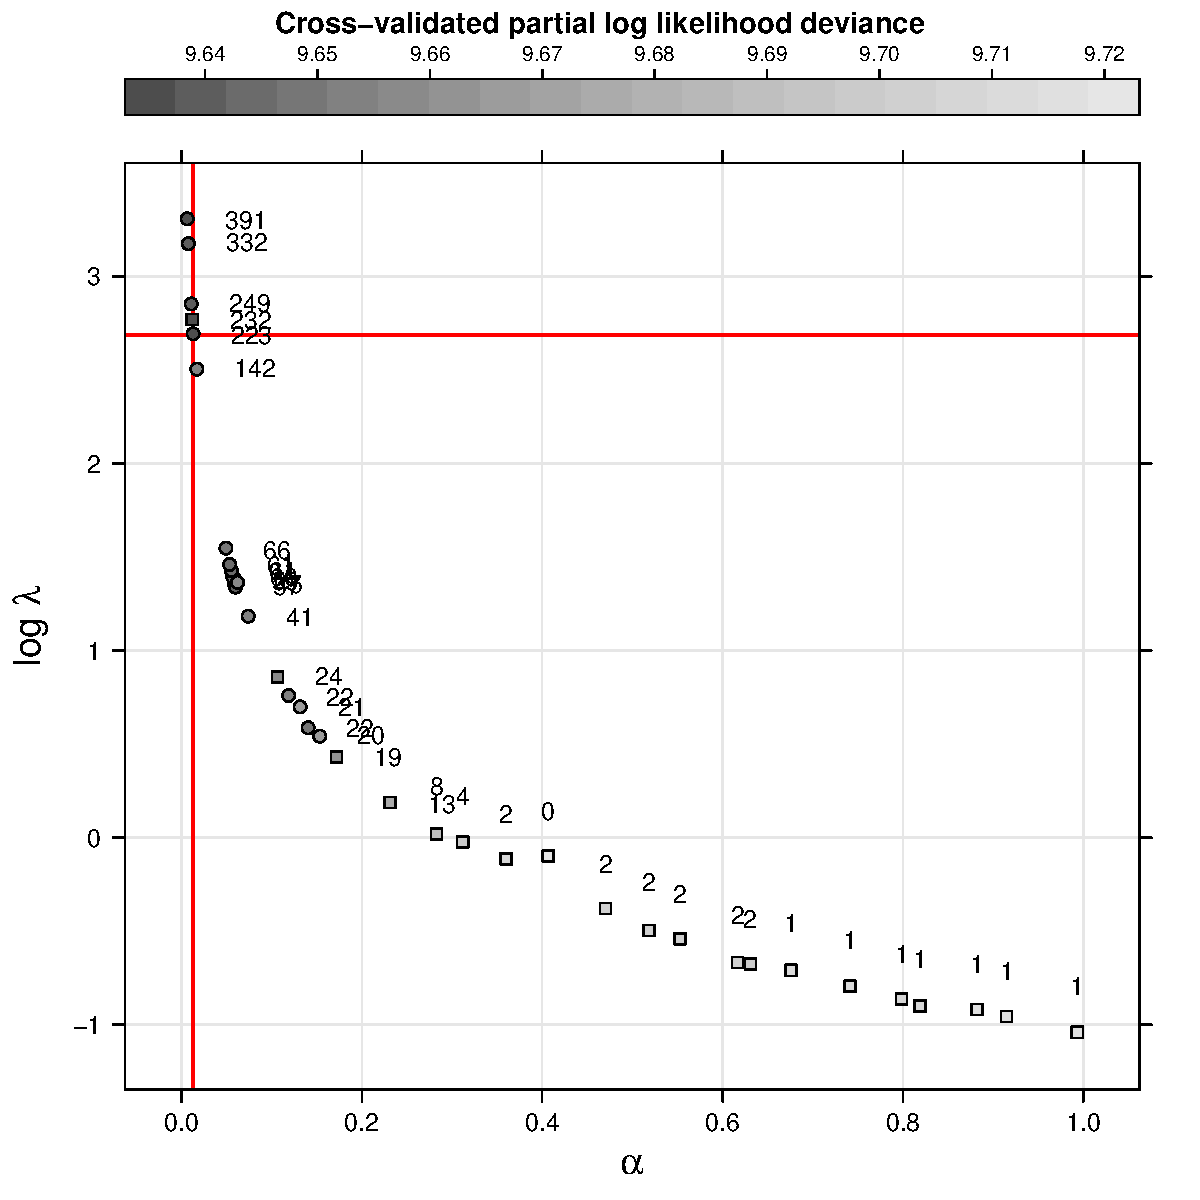
\includegraphics{c060_vignette-interval_search_cox_out_plot1}
\end{center}
\caption{Cross-validated partial log likelihood deviance as a function of both tuning parameters $\alpha$ and log$\lambda$ when fitting the elastic net Cox model for the AML data set. For each evaluated point in the parameter space the number of selected features in the corresponding model is printed next to the data point symbol. Rectangles correspond to initially selected $\alpha$ values. The solid red lines highlight the final solution where the loss function is within one standard error of the minimum. }
\label{fig:interval_search1}
\end{figure}

Figure~\ref{fig:interval_search1} illustrates the relationship between both tuning parameters $\alpha$ and $\lambda$ for the 'visited' points in the parameter space. The partial log likelihood deviance is  color-coded with black for small values and gray for large values.  The number of features selected  in the corresponding model is written near each point. 
To distinguish between initial and iteration points, the initial points are plotted as  squares and iteration points as circles. One can observe that the iteration points were chosen in the regions with lower deviance values.

The distribution of initial points (iteration=0) and visited points (iteration>0) in the parameter space is plotted in Figure~\ref{fig:interval_search2}.
This plot shows nicely that the interval search algorithm does not sequentially cover the entire parameter space, but rather quickly finds promising regions and draws new samples there. The optimal model contains with minimal log-likelihood deviance is found for $\alpha$ = 0.013 $\log\lambda$ = 2.689 and highlighted as a vertical line.

\begin{figure}[t!]
\begin{center}
\begin{Schunk}
\begin{Sinput}
R> plot(sumint,type="points") 
\end{Sinput}
\end{Schunk}
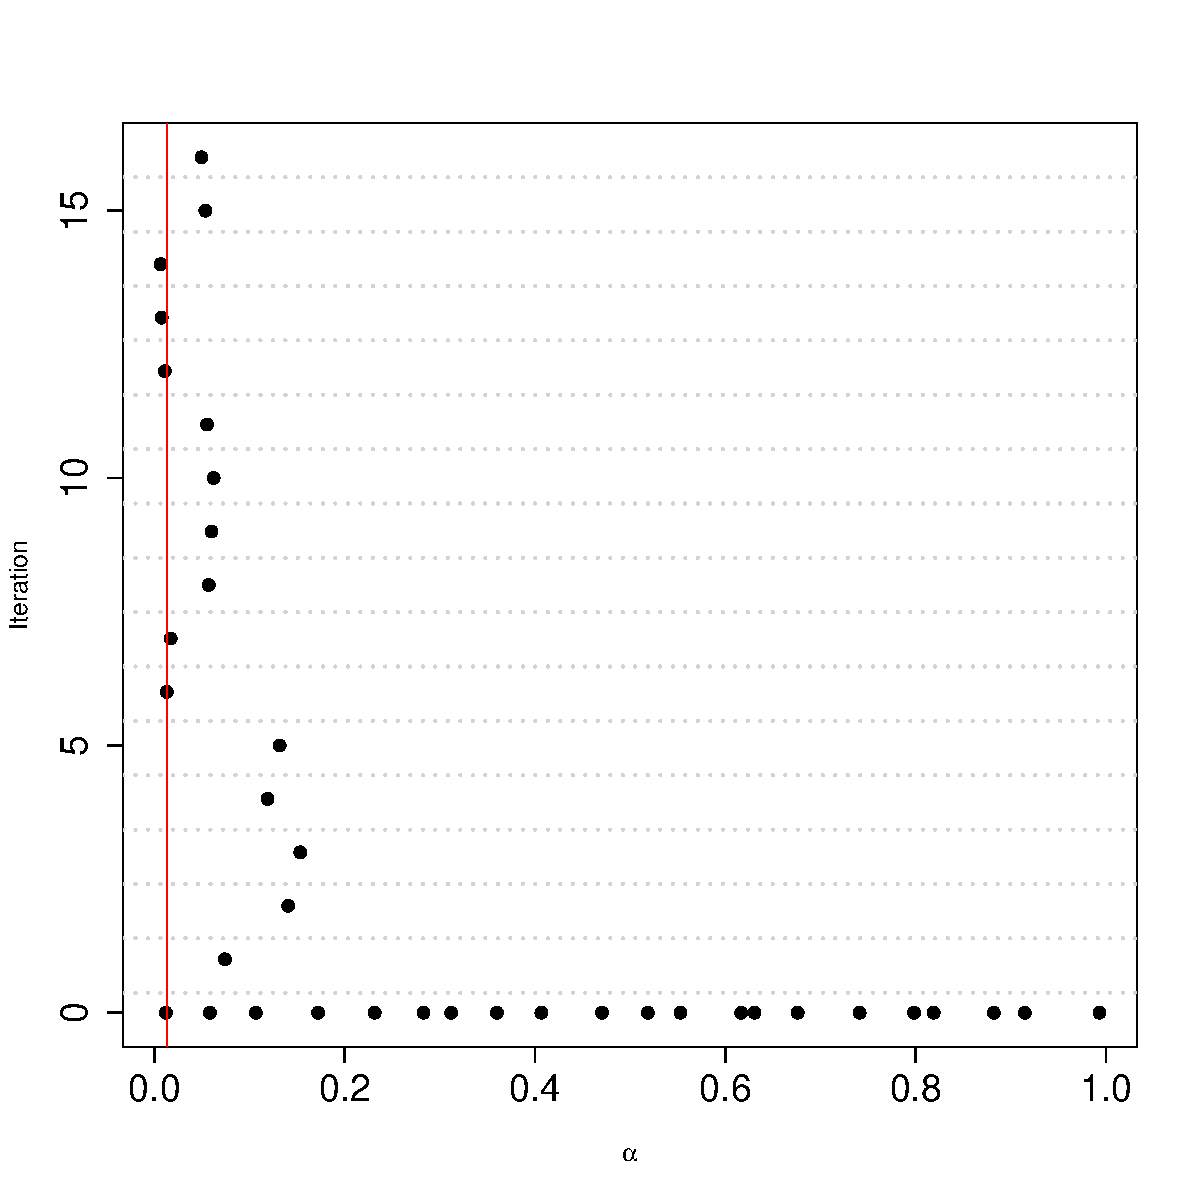
\includegraphics{c060_vignette-interval_search_cox_out_plot2}
\end{center}
\caption{The distribution of initial and visited points of the interval search plotted in chronological order. The interval search is employed to identify the optimal parameter value combination ($\alpha$,$\lambda$) for the elastic net Cox model fitted to the AML data set.}
\label{fig:interval_search2}
\end{figure}

To our knowledge, the interval search algorithm has not yet been applied for the purpose of optimizing the tuning parameters of elastic net models fitted with the \pkg{glmnet} package. The only previous \proglang{R} implementation of this approach was in the \proglang{R} package \pkg{penalizedSVM}, which implements classification and simultaneous feature selection with support vector machines. 

\begin{center}
\begin{table}
\small
\begin{tabular}{|p{4cm}|p{10cm}|l|l|}
\hline                        
Function & Description \\
\hline
\code{Plot.coef.glmnet} & Plot the \code{glmnet} coefficient path and highlight the path of a pre-specified set of variables\\
\hline
\code{PLL.coxnet} & Predictive partial log-likelihood for \code{glmnet} Cox PH model fit\\ 
\code{aggregation.auc} & Determine the area under the ROC curve for a fitted model\\
\code{complexity.glmnet} & Interface for determination of penalty \code{lambda} in \code{glmnet} models via cross-validation\\ 
\code{fit.glmnet} & Interface function for fitting a penalized regression model with \code{glmnet}\\
\code{Plot.peperr.curves} & Plot method for prediction error curves of a \code{peperr} object\\
\code{predictProb.coxnet} &  Extract predicted survival probabilities from a \code{coxnet} fit \\
\code{predictProb.glmnet} & Extract predicted survival probabilities from a \code{glmnet} fit \\
\hline
\code{stabpath} & Calculate the stability path for Gaussian, binomial, Poisson, multinomial and Cox \code{glmnet} models\\
\code{stabsel} & Estimate a stable set of variables and allows to control the PFER, PCER or FWER\\
\code{plot.stabpath} & Display stability path and indicates estimated stable features\\
\hline
\code{epsgo}              &Efficient Parameter Selection via Global Optimization\\
\code{summary.intsearch}  &Summary method for interval search models\\
\code{tune.glmnet.interval} &Wrapper function to apply \code{epsgo} to  \code{glmnet} objects\\
\code{plot.sum.intsearch} &Plot \code{sum.intsearch} objects generated by \code{summary.intsearch}\\
\hline
\end{tabular}
\caption{Overview of available functions in the \pkg{c060} package.}
\label{tab:functions}
\end{table}
\end{center}
%\clearpage
\section{Conclusions and outlook}
The programming language and statistical computing environment \proglang{R} provides a highly useful framework for statistical data analysis and modelling. It is the dominating statistical software in many areas, for example in molecular biology and molecular medicine, which is largely due to the highly successful Bioconductor project \citep{Bioconductor}, which provides tools for the analysis and interpretation of high-throughput genomic data. Due to the open-source nature of \proglang{R} and Bioconductor, many useful software packages have been developed by \proglang{R} users and made available for the \proglang{R} community. One example is the \pkg{glmnet} package, which  implements an efficient state-of-the-art algorithm for fitting penalized Cox and generalized linear models with lasso, ridge or elastic net penalties.

We have presented our \proglang{R} package \pkg{c060}, which provides extensions to \pkg{glmnet} and additional features, which are essential for a complete data analysis in real-life applications, including stability selection, estimation of prediction error (curves) and an efficient interval search algorithm for finding the optimal elastic net tuning parameter combination. These extensions have proved useful in our daily work, in particular for the task of performing prognostic modelling of patient survival data based on high-dimensional molecular biology data. Table \ref{tab:functions} lists all functions that are available as part of the \pkg{c060} package.

The \pkg{c060} package will be kept updated in the future to keep up with new developments in the field of penalized regression methodology for feature selection and risk prediction modelling with high-dimensional input data. One example are developments for the estimation of standard errors, confidence intervals and the determination of p-values in high-dimensional regularized regression models, e.g., through subsampling methods similar to the approach taken by \citet{wasserman2009} and \citet{MMB2009}.

\section*{Acknowledgments}

This work was partially funded by the Virtual Helmholtz Institute VH-VI-404.

%% include your article here, just as usual
%% Note that you should use the \pkg{}, \proglang{} and \code{} commands.

%\section[About Java]{About \proglang{Java}}
%% Note: If there is markup in \(sub)section, then it has to be escape as above.
%\clearpage
\bibliographystyle{jss}
\bibliography{c060}   % na
\end{document}
